% Cover pages and basic template importation requirements
% Change with your info -------------------------------------------------

\def\theauthor{Diogo Vala \newline Correia}
\def\thesistitle{Something about Smart Shelfs, UHF RFID and Item tagging}
\def\course{Master in Electronics and Telecommunications Engineering}

\def\orientador{José Alberto Fonseca}
\def\orientadord{Associated Professor at the Departamento de Enegenharia 
Electrónica e Telecomunica\c c\~oes of the University of Aveiro}

\def\coorientador{GHI}
\def\coorientadord{Professor Catedr\'atico da Universidade de Aveiro}

\def\president{ABC}
\def\presidentd{Professor Catedr\'atico da Universidade de Aveiro}

\def\vogal{KLM}
\def\vogald{Professor Catedr\'atico da Universidade de Aveiro}

\def\frontpic{assets/frontpic.jpg}

% Abstract and acknowledgements should be edited bellow following the
% example boilerplate

% -----------------------------------------------------------------------

\def\thedeclaration{
     Dissertation submitted to the University of Aveiro in fulfillment of the thesis
     requirement for the degree of \course, under the supervision of \orientador, \orientadord 
}

\TitlePage
  \HEADER{\BAR\FIG{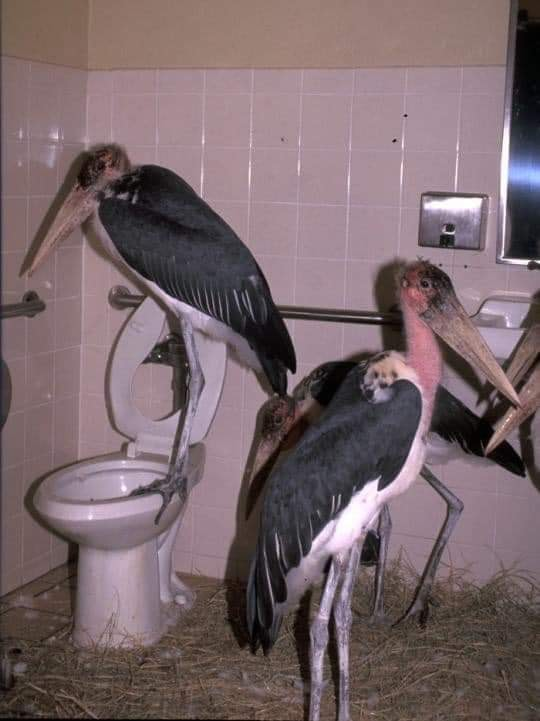
\includegraphics[height=100mm]{\frontpic}}} % the \FIG{} is optional
         {\ThesisYear}
  \TITLE{\theauthor}
        {\thesistitle}
\EndTitlePage
\titlepage\ \endtitlepage 

% Initial thesis pages
\TitlePage
  \HEADER{}{\ThesisYear}
  \TITLE{\theauthor{}}
        {\thesistitle}
  \vspace*{15mm}
  \TEXT{}
       {\thedeclaration}
\EndTitlePage
\titlepage\ \endtitlepage % empty page

\TitlePage
  \vspace*{55mm}
  \TEXT{\textbf{o j\'uri~/~the jury\newline}}
       {}
  \TEXT{presidente~/~president}
       {\textbf{\president}\newline {\small
        \presidentd \space (por delega\c c\~ao da Reitora da
        Universidade de Aveiro)}}
  \vspace*{5mm}
  \TEXT{vogais~/~examiners committee}
       {\textbf{\orientador}\newline {\small
        \orientadord \space (orientador)}}
  \vspace*{5mm}
  \TEXT{}
       {\textbf{\coorientador}\newline {\small
        \coorientadord \space (co-orientador)}}
  \vspace*{5mm}
  \TEXT{}
       {\textbf{\vogal}\newline {\small
        \vogald}}
\EndTitlePage
\titlepage\ \endtitlepage % empty page

\TitlePage
  \vspace*{55mm}
  \TEXT{\textbf{agradecimentos~/\newline acknowledgements}}
       {\'E com muito gosto que aproveito esta oportunidade para agradecer a todos os que me
        ajudaram durante este longos e penosos anos, cheios de altos e baixos (mais baixos que
        altos)\ldots}
  \TEXT{}
       {Desejo tamb\'em pedir desculpa a todos que tiveram de suportar o meu desinteresse pelas
        tarefas mundanas do dia-a-dia, \ldots}
\EndTitlePage
\titlepage\ \endtitlepage % empty page

\TitlePage
  \vspace*{55mm}
  \TEXT{\textbf{Resumo}}
       {Nos dias que correm, \'e frequente um trabalho ser avaliado pela sua apar\^encia em vez de
        o ser pelo seu conte\'udo. Sendo assim, sem descurar este \'ultimo, nesta tese descrevemos
        maneiras revolucion\'arias de transformar um documento s\'olido e austero num documento
        s\'olido e belo, capaz de fazer chorar de alegria (ou de inveja) qualquer leitor, mesmo
        quando este n\~ao percebe nada do que l\'a est\'a escrito.}
  \TEXT{}
       {A explora\c c\~ao de novas descobertas na \'area da percep\c c\~ao visual, nomeadamente
        no que se refere \`a aprecia\c c\~ao de obras de arte geniais, \ldots}
\EndTitlePage
\titlepage\ \endtitlepage % empty page

\TitlePage
  \vspace*{55mm}
  \TEXT{\textbf{Abstract}}
       {Nowadays, it is usual to evaluate a work \ldots}
\EndTitlePage
\titlepage\ \endtitlepage % empty page

% Tables of contents, of figures, ...

\pagenumbering{roman}
\tableofcontents

\cleardoublepage
\listoffigures

\cleardoublepage
\listoftables

\cleardoublepage
\printnoidxglossary[type=\acronymtype]
\addcontentsline{toc}{chapter}{\acronymname}

\cleardoublepage
\printnoidxglossary
\addcontentsline{toc}{chapter}{\glossaryname}

\cleardoublepage
\pagenumbering{arabic}